\paragraph{1.}
The main idea is to convert our problem into a network flow one, which we know we can solve in polynomial time.
To do so we give each directed edge a weight of one. Then we apply our network flow algorithm with source $s$ and sink $t$. This gives us an integer value $f$ of the maximum flow. We can show that there exist $k$ edge-disjoint directed path from $s$ to $t$ \textbf{iff} $f \geqslant k$.

It is easy to see that if there exist $k$ edge-disjoint directed path from $s$ to $t$, then by using this $k$ paths we will have a flow of $k$. Therefore the maximum flow is more than $k$.

Reciprocally, if $f \geqslant k$ then, as all edges have a weight of one, we can find $f$ edge-disjoint directed path from $s$ to $t$, only by using the edges that have a flow of one. Thus there exist $k$ edge-directed paths from $s$ to $t$.

\paragraph{2.}
We still want to apply a network flow algorithm but here there is some work to do with the graph to be able to do so. We are looking for node-disjoint paths, which means we need to ensure that each node can only see a flow of one. This can be done by duplicating all the nodes in our graph in order to separate the edges that are coming in a given node from the edges that are coming out. We then link the two duplicates by an edge of weight one so that the total flow in a node can be either one or zero (see figure \ref{fig2}).

Our new graph has $2|V|-2$ vertices and $|E|+|V|-2$ edges, so we can solve our problem in polynomial time using a network flow algorithm. It provides us with the value of the maximum flow $f$. We conclude using the fact that : there exist $k$ node-disjoint directed path from $s$ to $t$ \textbf{iff} $f \geqslant k$.

\begin{figure}[H]
\centering

\includegraphics[width=14cm]{fig2.png}
\caption{Graph transformation for a node}
\label{fig2}
\end{figure}


\paragraph{3.}
Here we need to reason in terms of min-cut and use the max-flow min-cut theorem to do the link with the property proved in question 1.

Let's suppose that we have a cut $C$ between $s$ and $t$ such that its value $c$ is strictly less than $k$ : $c < k$.
Let's prove that we can construct a cut of value $c$ either between $s$ and $u$ or between $u$ and $t$. Our cut $C$ is able to separate either $s$ and $u$ or $u$ and $t$. By the property of question 1., this violates the hypothesis :"there exist $k$ edge-disjoint paths from $s$ to $u$ and re-exist $k$ edge-disjoint paths from $u$ to $t$".

This proves that the minimal cut between $s$ and $t$ has a value of at least $k$, which concludes the proof :

If there exist $k$ edge-disjoint paths from $s$ to $u$ and re-exist $k$ edge-disjoint paths from $u$ to $t$, then there does exist $k$ edge-disjoint directed paths from $s$ to $t$.





\paragraph{4.}
Here is a counter-example.

\begin{figure}[H]
\centering
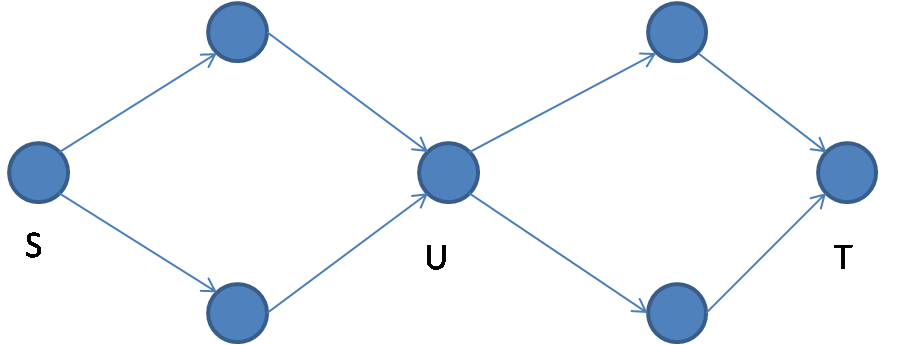
\includegraphics[width=8cm]{fig4b.png}
\caption{Counter-example with $k=2$}
\label{fig4}
\end{figure}